\documentclass[a4paper,14pt]{extarticle}
\usepackage[utf8]{inputenc}
\usepackage[english,russian]{babel}
\usepackage{makecell}
\usepackage{amsthm}
\usepackage{graphicx}
\usepackage{caption}
\usepackage{amssymb}
\usepackage{amsmath}
\usepackage{mathrsfs}
\usepackage{euscript}
\usepackage{graphicx}
\usepackage{subfig}
\usepackage{caption}
\usepackage{color}
\usepackage{bm}
\usepackage{tabularx}
\usepackage{adjustbox}
\usepackage{multirow}
\usepackage{xcolor}
\usepackage{url}
\usepackage{hyperref}


\usepackage[toc,page]{appendix}

\usepackage{comment}
\usepackage{rotating}

\DeclareMathOperator*{\argmax}{arg\,max}
\DeclareMathOperator*{\argmin}{arg\,min}

\newtheorem{theorem}{Теорема}
\newtheorem{lemma}[theorem]{Лемма}
\newtheorem{definition}{Определение}[section]

\numberwithin{equation}{section}

\newcommand*{\No}{No.}

\begin{document}

% Титульный лист
%\begin{titlepage}
    	\begin{center}
        		Министерство науки и высшего образования Российской Федерации Федеральное государственное автономное образовательное учреждение высшего образования
       
		«Московский физико-технический институт (национальный исследовательский институт)»

        		Факультет управления и прикладной математики\\
        		Кафедра <<Интеллектуальные системы>>\\
    	\end{center}

    	\vspace{2cm}

    	\begin{center}
       		\Large \bf Анализ свойств локальных моделей в задачах кластеризации временных рядов
    	\end{center}
    
    	\begin{center}
		~\\[-28pt]
		Выпускная квалификационная работа\\
		(бакалаврская работа)
	\end{center}
	
	\vspace{0.1cm}
	    
    \begin{center}
    	\textbf{Направление подготовки:} 03.03.01 Прикладные математика и физика
    \end{center}

   \vspace{0.1cm}

	\begin{flushright}
		\begin{table}[!ht]
			\centering
			\begin{tabular}{l}
				~~~~~~~~~~~~~~~~~~~~~~~~~~~~~~~~~~~~~~~~~~~~~~~~~~ \textbf{Выполнил:}\\
				~~~~~~~~~~~~~~~~~~~~~~~~~~~~~~~~~~~~~~~~~~~~~~~~~~ студент группы 574\\
				~~~~~~~~~~~~~~~~~~~~~~~~~~~~~~~~~~~~~~~~~~~~~~~~~~ Грабовой Андрей Валериевич\\
				~~~~~~~~~~~~~~~~~~~~~~~~~~~~~~~~~~~~~~~~~~~~~~~~~~ \underline{\hspace{7cm}}\\[-10pt]
				\begin{scriptsize}
	    			~~~~~~~~~~~~~~~~~~~~~~~~~~~~~~~~~~~~~~~~~~~~~~~~~~~~~~~~~~~~~~~~~~~~~~~~~~~~~~~~~~~~~~~~~~~~~~~~~~\,
	    			(подпись обучающегося)
	   		 	\end{scriptsize}\\[15pt]
				~~~~~~~~~~~~~~~~~~~~~~~~~~~~~~~~~~~~~~~~~~~~~~~~~~ \textbf{Научный руководитель:}\\
				~~~~~~~~~~~~~~~~~~~~~~~~~~~~~~~~~~~~~~~~~~~~~~~~~~ Доктор физико-математических наук\\
				~~~~~~~~~~~~~~~~~~~~~~~~~~~~~~~~~~~~~~~~~~~~~~~~~~ Стрижов Вадим Викторович\\
				~~~~~~~~~~~~~~~~~~~~~~~~~~~~~~~~~~~~~~~~~~~~~~~~~~ \underline{\hspace{7cm}}\\[-10pt]
				\begin{scriptsize}
					~~~~~~~~~~~~~~~~~~~~~~~~~~~~~~~~~~~~~~~~~~~~~~~~~~~~~~~~~~~~~~~~~~~~~~~~~~~~~~~~~~~~~~~~~~~~
	    			(подпись научного руководителя)
	    		\end{scriptsize}
	    	\end{tabular}
	    \end{table}
	\end{flushright}


	\begin{center}
		Москва 2019
	\end{center}

\end{titlepage}




% Аннотация
\newpage


\begin{abstract}
В данной работе представлены два исследования, посвящённые задаче исправления грамматических ошибок в текстах с использованием подхода Sequence Tagging. В первом исследовании описывается адаптация модели GECToR для русского языка. С учетом недостатка размеченных данных, для обучения модели был создан синтетический набор данных. Разработанная модель показала хорошие результаты на синтетических данных $F_{0.5}$ = 82.5, а также продемонстрировала способность к переносу знаний на тестовый набор данных RULEC без дополнительного обучения $F_{0.5}$ = 22.2.

Во втором исследовании предлагается полностью автоматизированный, не требующий разметки подход к решению задачи исправления грамматических ошибок. Метод основан на генерации данных с использованием алгоритма Левенштейна для исправления грамматических ошибок на уровне подслов с использованием правил: keep, append, replace и delete. Подход универсален для любого языка и не требует дополнительной разметки. Применение данного метода к оригинальной модели GECToR позволило достичь конкурентных результатов на английском языке: $F_{0.5}$ = 62.4 на CoNLL-2014 и $F_{0.5}$ = 61.9 на BEA-2019, при этом не потребовалось ни аннотирования данных, ни составления словаря грамматических правил.

Таким образом, совместное рассмотрение обоих исследований демонстрирует возможности применения и адаптации Sequence Tag-ging моделей как для языков с достаточным количеством размеченных данных, так и для языков, где количество таких данных ограничено.

\smallskip
\textbf{Ключевые слова}: исправление грамматических ошибок; обработка естественного языка; алгоритм левенштейна; трансформер.
\end{abstract}






% Нумерация должна начинаться со второй страницы
\setcounter{page}{2}

% Оглавление
\newpage
\tableofcontents

% Обозначения и сокращения
% \input{./dict.tex}

% Введение
\newpage


\section{Введение}
% В современном мире проблема автоматического исправления грамматических ошибок (ИГО) является актуальной~\cite{b1, b2, b3} в связи с увеличением объема текстовых данных~\cite{b4}. Ручная проверка больших текстов является трудоемкой задачей. Кроме того, решение данной задачи имеет специфические приложения: проверка сочинений~\cite{b5}; исправление сообщений в социальных сетях~\cite{b6}; исправление текстов, написанных иностранными студентами~\cite{b7}; поиск текстовых заимствований~\cite{b8}. Последнее объясняется тем, что грамматические ошибки являются одним из способов обхода системы поиска текстовых заимствований~\cite{b9}. Для обучения моделей поиска текстовых заимствований используются тексты научных статей, содержащие небольшое количество ошибок. Пользователи при этом могут нарочно допускать множество ошибок, влияя тем самым на предсказания модели. Это приводит к появлению состязательных атак (англ. adversarial attacks) на модели обработки естественного языка~\cite{b10}. Большинство исследований в области ИГО ориентировано на английский язык~\cite{b11}. Для многих других языков, включая русский, число исследований значительно меньше~\cite{b12}. Особенно стоит отметить сложную морфологию русского языка, что усложняет решение задачи ИГО.
% В настоящее время существует два наиболее эффективных подхода решения задачи ИГО для английского языка, – Sequence-to-Sequence (Seq2Seq)~\cite{b13, b14} и Sequence Tagging (ST)~\cite{b15, b16}. В подходе Seq2Seq исходная последовательность представляет собой предложение с ошибками, а целевая последовательность – предложение без ошибок. Такой подход решения задачи ИГО работает хорошо, но обладают низкой скоростью работы, а также плохой интерпретируемостью, поскольку для определения типа ошибки необходимо использовать дополнительный функционал. Модели, основанные на подходе ST, не имеют данных проблем: не требуется полностью генерировать предложение без ошибок, достаточно лишь отметить ошибки в исходном предложении. Кроме того, они легко интерпретируемы, так как решают задачу классификации для каждого токена, сопоставляя ему нужное правило из заданного словаря корректирующих правил. Таким образом, для объяснения исправления, применяемого к токену, не требуется дополнительный функционал.
% В~\cite{b12} авторы сравнивают данные подходы для решения задачи ИГО в текстах на русском языке. Результаты показывают, что на небольшом объеме размеченных данных методы, основанные на подходе ST, существенно превосходят методы, основанные на подходе Seq2Seq. Для сравнения методов авторы представляют набор данных RULEC, содержащий предложения с размеченными грамматическими ошибками. Набор данных состоит из сочинений иностранных студентов.
% Для решения задачи ИГО на английской языке наиболее эффективной ST-моделью является GECToR~\cite{b15}. Данная модель состоит из кодировщика на основе архитектуры трансформер~\cite{b17} и двухголового классификатора. Авторы статьи провели сравнение использования моделей BERT~\cite{b18}, RoBERTa~\cite{b19} и XLNet~\cite{b20} в качестве кодировщиков. Первая голова предсказывает наличие ошибки, а вторая – соответствующее правило для исправления ошибки. После этого соответствующее правило применяется к каждому токену последовательности для исправления. Если токен не содержит ошибок, то данному токену ставится в соответствие правило “\$KEEP”, которое оставляет данный токен без изменений. Обучение модели GECToR состоит из трех этапов: 
% \begin{enumerate}
%     \item обучение на синтетических данных;
%     \item дообучение на корпусе данных, содержащем ошибки;
%     \item дообучение на комбинации из корпусов данных с ошибками и без ошибок.  
% \end{enumerate}
% В рамках магистерской диссертации были проделаны два основных исследования:
% \begin{enumerate}
%     \item в работе предложен алгоритм генерации синтетического набора
% данных, содержащего тексты на русском языке для первого этапа обучения. Модель GECToR адаптирована в модель RuGECToR~\cite{b21} для ИГО в русскоязычных текстах с использованием сгенерированных синтетических данных и данных из открытых источников. Данная модель не требует большого количества данных для обучения, в отличие от моделей на основе архитектуры Seq2Seq, и показывает конкурентноспособное качество для английского языка. Целью данного исследования является обучение модели, способной обобщать морфологические свойства русского языка, а не подстраиваться под обучающую выборку;
%     \item в рамках второго исследовании мы предложили методику автоматического построения словаря корректирующих правил и обучения с помощью него ST-моделей. Наш подход основан на переходе к уровню SentencePiece-токенов~\cite{b22} в GEC. Мы использовали только “базовые преобразования”, общие для всех языков – \textit{keep}, \textit{append}, \textit{replace} и \textit{delete}.  Таким образом, мы полностью избавились от грамматических зависимостей. Для экспериментов мы применили наш подход к ST-модели GECToR. Мы показали, что такой метод дает сопоставимые по качеству результаты, при этом является полностью автоматическим. Кроме того, этот подход можно адаптировать к любому языку, поскольку он не требует знания грамматических правил или ручных аннотаций.
% \end{enumerate}

В настоящее время задача автоматической коррекции грамматических ошибок приобретает всё большую значимость~\cite{b1, b2, b3}, что связано с ростом объёмов текстовой информации~\cite{b4}. Проверка больших текстов вручную требует значительных затрат времени и усилий. Таким образом, исследования в данной области необходимы для автоматизации данных процеессов. Например, при проверке письменных работ~\cite{b5} преподаватели тратят большое количество времени на оценку каждого ученика, хотя было бы менее трудоемко для первичной оценки использовать автоматический алгоритм, а далее валидировать полученный результат с помощью учителя. Сюда же относится и проверка грамотности в социальных сетях --- хотя автоматическая проверка орфографии уже существует, исправление грамматики до сих пор остаётся нерешённой задачей~\cite{b6}. Это может быть использовано не только для социальных сетей, но и для разработки приложения по изучению языков --- редактирование текстов, созданных иностранными студентами~\cite{b7} Также намеренные грамматические ошибки могут использоваться для обхода систем обнаружения плагиата~\cite{b8, b9}. Это приводит к возникновению состязательных атак на модели обнаружения плагиата~\cite{b10}, которые изначально обучались на наборах данных, содержащих минимальное количество ошибок. 

В настоящее время большинство методов автоматического исправления грамматики ориентированы на английский язык~\cite{b11}, где подобные системы показывают высокую эффективность. В то время как для других языков, включая русский, количество исследований остается ограниченным~\cite{b12}. Основная сложность заключается в морфологическом богатстве русского языка, что создает существенные препятствия для разработки эффективных систем коррекции грамматических ошибок.

% Среди наиболее результативных подходов к автоматическому исправлению грамматических ошибок для английского языка можно выделить два: Sequence-to-Sequence (Seq2Seq)~\cite{b13, b14} и Sequence Tagging (ST)~\cite{b15, b16}. В рамках Seq2Seq-методов модель получает на вход предложение с ошибками и генерирует правильный вариант. Хотя такие модели демонстрируют высокое качество исправлений, они обладают рядом недостатков: низкая скорость обработки и сложность интерпретации, так как для выявления типов ошибок требуется дополнительный анализ. Подход ST лишён этих недостатков: он не требует полной генерации исправленного текста, а лишь помечает и исправляет ошибки в исходной последовательности. К тому же, модели ST лучше интерпретируемы, так как каждая ошибка классифицируется и соотносится с конкретным правилом из словаря исправлений, что делает объяснение корректировок прозрачным.

Среди наиболее эффективных подходов к автоматическому исправлению грамматических ошибок в английском языке выделяются две основные архитектуры: Sequence-to-Sequence (Seq2Seq)~\cite{b13, b14} и Sequence Tagging (ST)~\cite{b15, b16}.

Модели типа Seq2Seq работают по принципу “чёрного ящика”: на вход подаётся ошибочное предложение, а на выходе генерируется исправленный вариант. Несмотря на высокую точность таких систем, они имеют существенные ограничения:

\begin{enumerate}
    \item низкая производительность из-за вычислительной сложности полной генерации текста;
    
    \item слабая интерпретируемость результатов, требующая дополнительного анализа для определения типов ошибок.
\end{enumerate}

В то время как при использовании моделей на основе архитектуры ST исправление происходит на уровне токенов, ошибки помечаются и корректируются в исходной последовательности без полной перегенерации текста. Также данное решение является более интепретируемым, поскольку каждое исправление соотносится с конкретным грамматическим правилом из словаря. Также с точки зрения эффективности обеспечивается лучшая производительность за счёт локального характера исправлений

В исследовании~\cite{b12} проводится сравнительный анализ данных подходов на материале русскоязычных текстов. Результаты показывают, что ST-модели значительно превосходят Seq2Seq при ограниченном объеме размеченных данных. Эксперименты выполнены на корпусе RULEC, который был разработан авторами исследования. Набор данных состоит из предложений иностранных студентов с аннотированными грамматическими ошибками. Данный корпус был использован для оценки работы нашей модели в экспериментах, но не был использован для ее обучения. 


GECToR~\cite{b15} в настоящее время считается одной из наиболее эффективных ST-моделей для английского языка. Модель построена на основе архитектуры трансформер~\cite{b17} и использует двухголовый механизм классификации. Первая голова отвечает за детекцию ошибок, вторая — за определение типа исправления. Если ошибка не обнаружена, применяется специальная метка “\$KEEP”, сохраняющая исходный токен без изменений. В экспериментах были рассмотрены различные кодировщики: BERT~\cite{b18}, RoBERTa~\cite{b19} и XLNet~\cite{b20}. Обучение модели проводилось в три этапа: обучение на синтетических данных, дообучение на корпусе с ошибками и дообучение на объединённом корпусе с ошибками и без них.

В рамках магистерской работы были выполнены два ключевых исследования:
\begin{enumerate}
    \item В рамках первого исследования был разработан алгоритм генерации синтетических данных для русского языка. На его основе создана русскоязычная адаптация модели GECToR — RuGECToR~\cite{b21}. Хотя обучение проводилось исключительно на синтетических данных, модель была ориентирована на выявление и обобщение грамматических закономерностей русского языка, а не на простое запоминание примеров.
    \item Предложен способ автоматического построения словаря корректирующих правил и последующего обучения ST-моделей с его использованием. Метод опирается на уровень SentencePiece-токенов~\cite{b22} и ограничивается универсальными преобразованиями: \textit{keep}, \textit{append}, \textit{replace} и \textit{delete}. Такой подход позволяет устранить зависимость от грамматических правил, полностью автоматизируя процесс. Метод был реализован на примере модели GECToR и показал сопоставимые результаты, при этом обеспечивая лёгкую адаптацию к другим языкам без необходимости ручной аннотации или знаний грамматики.
\end{enumerate}




% Введение
\newpage

\section{Адаптация модели GECToR для русского языка}
\subsection{Постановка задачи}

Задано множество пар, в котором каждая пара состоит из предложения \( x_i \) и соответствующего ему эталонного исправления \( t_i \):
\[
S = \{(x_i, t_i)\}_{i=1}^N,
\]
где \( N \) – количество пар. 

В данной работе предполагается, что каждое предложение представлено в виде последовательности токенов \( x_i = \{s_1, s_2, \dots, s_{n_i}\} \), а каждое эталонное исправление – в виде последовательности корректирующих правил \( t_i = \{t_1, t_2, \dots, t_{n_i}\} \), где \( n_i \) – длина \( i \)-го предложения. 

Под понятием <<токен>> подразумевается слово, таким образом разбиение предложения на токены происходит на уровне слов. Каждое корректирующее правило \( t_j \) является элементом заданного нами словаря. Составление словаря описано ниже.

Целью задачи является нахождение функции \( T \) для построения отображения из последовательности токенов \( x_i \) в последовательность корректирующих правил \( t_i \):
\[
T: x_i \mapsto t_i \in \{0, 1, \dots, k\}^{n_i},
\]
где \( k \) – размер словаря корректирующих правил.
 



% Введение
\newpage

\subsection{Предлагаемый подход}

На вход модели GECToR подается предложение, которое требуется исправить. Далее предложение разбивается на последовательность токенов. Таким образом, задача исправления грамматических ошибок сводится к нахождению отображения \( T \) для сопоставления каждого токена с соответствующим правилом из словаря корректирующих правил. Для русского языка построен словарь, состоящий из 5183 правил, которые будут подробно описаны ниже.

Данная постановка задачи имеет недостаток: каждый токен сопоставляется только с одним правилом из словаря, но иногда для исправления ошибки требуется большее количество изменений. Для решения данной проблемы предлагается использовать итеративное исправление: предложение, полученное в результате работы модели, снова подается модели на вход. Таким образом, модель предсказывает правила для новой последовательности токенов. Правила разработаны таким образом, что последовательность токенов с ошибками может быть преобразована в последовательность токенов без ошибок за конечное число итераций. Проделаны следующие адаптации модели GECToR для русского языка:


\begin{enumerate}
    \item Проведено обучение модели RUGECToR в два этапа:
    \begin{enumerate}
        \item обучение на синтетических данных с ошибками;
        \item дообучение на комбинации из синтетических данных с ошибками и без ошибок;
    \end{enumerate}
    
    \item Изменен этап применения модели для исправления ошибок с использованием библиотеки pymorphy2~\cite{b23};
    
    \item Составлен словарь правил для исправления ошибок;
    
    \item В качестве кодировщика использован Multilingual BERT.

    
\end{enumerate}

% Введение
\newpage


\subsection{Описание набора данных}

\newcommand{\RomanNumeralCaps}[1]{\MakeUppercase{\romannumeral #1}}

\begin{table*}[ht!]
\fontsize{10pt}{12pt}\selectfont
\centering
\begin{tabular}{| p{4.5cm} | p{4.5cm} | p{6cm} |}
  \hline
  \textbf{исходное предложение}  & \textbf{предложение с ошибками} & \textbf{корректирующие правила} \\ 
  \hline
  \foreignlanguage{russian}{\textcolor{red}{'Человеческий', 'дух'}, 'непостижимо', 'могуч', ',', и', 'убить', 'его', 'в', \textcolor{red}{'человеке'}, 'почти', 'невозможно', '.'}
  & \foreignlanguage{russian}{\textcolor{red}{'Человеческий-дух'}, 'непостижимо', 'могуч', ',', 'и', 'убить', 'его', 'в', \textcolor{red}{'чел овеке'}, 'почти', 'невозможно', '.' }
  & {\textcolor{red}{\$TRANSFORM\_SPLIT\_HYPHEN}, \$KEEP, \$KEEP, \$KEEP,
  \$KEEP, \$KEEP, \$KEEP, \$KEEP, \textcolor{red}{\$MERGE\_SPACE}, \$KEEP, \$KEEP, \$KEEP, \$KEEP} \\ 
  \hline
\end{tabular}
\caption{Пример генерации ошибок в предложении}
\label{tab1}
\end{table*}

Для генерации синтетических ошибок на первом этапе обучения взяты предложения из русскоязычной Википедии и школьных сочинений~\cite{b24}. Для второго этапа обучения использованы школьные сочинения и литературные тексты~\cite{b25}. Сгенерированы специализированные ошибки для следующих частей речи: глагол, имя прилагательное, имя существительное, местоимение, причастие и числительное. Перед началом процесса генерации ошибок пронумерованы позиции токенов для указанных частей речи во всех предложениях.
Процесс генерации ошибок осуществляется следующим образом: 
\begin{enumerate}
    \item случайным образом выбирается предложение, где для каждого токена случайным образом генерируется ошибка, соответствующая части речи токена;
    \item после этого каждому такому токену ставится в соответствие правило из словаря корректирующих правил, которое необходимо применить для исправления ошибки.
\end{enumerate}
Распределение ошибок близко к равномерному. В табл.~\ref{tab1} показан пример генерации ошибок в предложении.


\begin{table}[ht!]
\begin{center}
\begin{tabular}{|l|c|c|c|}
  \hline
  \textbf{набор данных} & \textbf{\#предложений} & \makecell{\textbf{\% предложений} \\ \textbf{с ошибками}} & \makecell{\textbf{этап} \\ \textbf{обучения}} \\ \hline
  Wiki + Essays & $10\,000\,000$ & $\approx 100\%$ & \RomanNumeralCaps{1} \\ \hline
  Proza + Essays & $1\,000\,000$ & $\approx 50\%$ & \RomanNumeralCaps{2} \\ \hline
\end{tabular}
\caption{Информация об обучающем наборе данных}
\label{tab2}
\end{center}
\end{table}


В табл.~\ref{tab2} показано, что для первого этапа обучения использовалось 10.000.000 предложений, где каждое предложение содержит произвольные типы ошибок кроме пунктуационных. Для второго этапа обучения мы использовали 1.000.000 предложений: 500.000 предложений не содержат ошибок; 250.000 предложений содержат все ошибки, кроме пунктуационных; оставшиеся 250.000 предложений содержат только пунктуационные ошибки. Для проведения второго этапа обучения добавлены литературные произведения и исключена Википедия с целью сделать модель более устойчивой к различиям между наборами данных~\cite{b26}. В качестве тестовых наборов данных использовались школьные сочинения и тестовое подмножество набора данных RULEC. 
В работе~\cite{b15} авторы разделяют правила, применяемые к исходным токенам $\{x_1,x_2,…,x_{n_i} \}$ для получения целевого предложения, на два типа – базовые и грамматические. В нашем исследовании сохранено данное разделение. Грамматические правила подобраны таким образом, чтобы словарь корректирующих правил покрывал множество правил русского языка. Базовые правила выполняют наиболее распространенные операции редактирования на уровне токенов: сохранение текущего токена $x_i$ без изменений – правило $\$KEEP$, удаление текущего токена $x_i$ – правило $\$DELETE$, добавление нового токена $t_1$ после текущего токена $x_i$ – правило $\$APPEND\_t_1$ или замена текущего токена $x_i$ на другой токен $t_2$ – правило $\$REPLACE\_t_2$. Для генерации правил \$APPEND и \$REPLACE использованы 2500 наиболее употребляемых русских слов с точки зрения коэффициента Жуайна~\cite{b27}. Для каждого слова $w_i$ добавлены соответствующие правила $\$APPEND\_w_i$ и $\$REPLACE\_w_i$.
Грамматические правила выполняют операции, специфичные для конкретного случая. Для русского языка использованы следующие правила, которые применяются непосредственно к токену: изменение времени, падежа, рода, лица и числа. Добавлены правила для часто допускаемых ошибок, например, правописание “ться”/“тся” и “при”/“пре”. Также использованы правила, которые не зависят от языка: объединение двух слов с помощью пробела или дефиса; разделение слова, написанного через дефис, на две части; изменение регистра первой буквы слова.
Рассмотрим пример корректирующего правила для исправления “красивая” на “красивый”. Таким образом, необходимо преобразовать прилагательное из женского рода в мужской. Изначально правила для грамматических преобразований создавались следующим образом:
\begin{center}
\$TRANSFORM\_{\color{orange} ADJF}\_GEND\_{\color{orange} femn}\_masc
\end{center}
Такие правила содержали подробную информацию о:
\begin{enumerate}
    \item части речи слова; 
    \item грамматическом признаке, который необходимо изменить; 
    \item граммеме как для исходного, так и для исправленного слова.
\end{enumerate}
 Далее было решено объединить правила для разных частей речи, исключив название части речи. Кроме того, решено отказаться от указания граммемы для исходного (неправильного) слова, поскольку для его исправления необходима информация только о новой граммеме. В данном исследовании предполагается, что модель сама научится сопоставлять правила соответственно частям речи. Например, глагол и прилагательное могут менять род, а существительное – нет. Таким образом, итоговые правила, используемые в нашей модели, выглядят следующим образом:
 \begin{center}
\$TRANSFORM\_GEND\_masc
\end{center}
Данная модификация была сделана для того, чтобы уменьшить размер словаря и увеличить количество примеров для каждого правила в обучающем наборе данных. Таким образом достигается компромисс между обобщающей способностью и размером модели, так как с ростом количества правил увеличивается размер слоя классификации. 

Для оценки полноты составленного набора правил было проведено сравнение с классификатором ошибок в наборе данных RULEC. Для большинства ошибок из набора данных RULEC в нашем словаре существуют аналогичные правила. Но в наборе данных RULEC существуют и более узкие правила, например, “Местоимение’’, “Сущ.: число”, означающие наличие ошибки в написании множественного/ единственного в соответствующих частях речи. Для данных ошибок в нашем словаре нет специализированных правил, но тем не менее они покрываются более широкими правилами для исправления написания множественного/единственного числа без привязывания к конкретным частям речи. Также существуют правила, такие как “Орфография”, “Союз” и “Предлог”, аналогов которым нет в нашем словаре. Исправление ошибок, связанных с данными правилами, предусмотрено правилами $\$APPEND\_w_i$ и $\$REPLACE\_w_i$.

\subsection{Эксперименты}
В качестве предобученного кодировщика на основе архитектуры трансформер выбран Multilingual BERT~\cite{b28}, имеющий хорошую языковую обобщаю способность. Эксперименты по сравнению различных кодировщиков на основе архитектуры трансформер запланированы в дальнейших работах. Обучение модели проводилось в течение двух этапов, каждый из которых длился 50 эпох. На первом этапе обучения размер батча равен 32, на втором – 16. В качестве оптимизатора параметров выбран Adam с параметром $lr=10^{-5}$. 
Для работы модели на этапе применения было выявлено, что количество исправлений уменьшается с каждой успешной итерацией, и необходимое число исправлений выполняется в течение первых трех итераций. 

\subsection{Метрики качества}

Сравнение качества работы моделей проводилось на синтетических и реальных данных. Для оценки качества использованы метрики, описанные в\cite{b11}:

\begin{equation*}
    R = \frac{\sum_{i=1}^{N} |g_i \cap e_i|}{\sum_{i=1}^{N} |g_i|}, \quad
    P = \frac{\sum_{i=1}^{N} |g_i \cap e_i|}{\sum_{i=1}^{N} |e_i|},
\end{equation*}
\begin{equation*}
    F_{0.5} = \frac{(1 + 0.5^2) \cdot R \cdot P}{R + 0.5^2 \cdot P},
\end{equation*}

где $N$~-- количество предложений, $e_i$~-- множество исправлений, предсказанных нашей моделью для предложения $s_i$, а $g_i$~-- множество эталонных исправлений. Пересечение между $g_i$ и $e_i$ определяется как:

\begin{equation*}
    g_i \cap e_i = \{ e \in e_i \mid \exists g \in g_i \colon e = g \}.
\end{equation*}




\subsection{Результаты}


\begin{table}[ht!]
\begin{center}
\begin{tabular}{|l|l|l|l|l|}
  \hline
  System & Training stage & $P$ & $R$ & $ F_{0.5} $\\ \hline
  RuGECToR & \RomanNumeralCaps{1} & 88.4 & 67.1 & 83.1 \\ \hline
  RuGECToR & \RomanNumeralCaps{2} & 88.5 & 65.1 & 82.5 \\ \hline
\end{tabular}
\caption{Качество работы модели на синтетическом тестовом наборе данных}
\label{tab3}
\end{center}
\end{table}

Для синтетического тестового набора данных сгенерировано 10.000 предложений с ошибками. Результаты на синтетическом наборе данных приведены в табл.~\ref{tab3}. Видно, что метрики $R$ и $F_{0.5}$ на втором этапе обучения ниже, чем на первом. Это можно объяснить двумя причинами:
\begin{enumerate}
    \item 50\% предложений в данных, использованных для второго этапа обучения, не содержали ошибок. Точность стала выше, но при этом количество охватываемых токенов уменьшилось.
    \item На втором этапе обучения были использованы дополнительные предложения из литературных произведений, которые не использовались во время первого этапа обучения. Таким образом, была увеличена обобщающая способность модели за счет добавления данных из другого распределения.
\end{enumerate}

\begin{table}[ht!]
\begin{center}
\begin{tabular}{|l|l|l|l|l|}
  \hline
  модель & данные для обучения data & $P$ & $R$ & $ F_{0.5} $\\ \hline
  Classifiers (learner) & RULEC & 22.6 & 4.8 & 12.9 \\ \hline
  Classifiers (min sup.) & RULEC & 38.0 & 7.5 & 21.0 \\ \hline
  MT & RULEC & 30.6 & 2.9 & 10.6 \\ \hline
  RuGECToR & Synthetic (\RomanNumeralCaps{1} stage) & 23.6 & 5.6 & 14.3 \\ \hline
  RuGECToR & Synthetic (\RomanNumeralCaps{2} stages) & \textbf{40.8} & \textbf{7.9} & \textbf{22.2} \\ \hline
\end{tabular}
\caption{Сравнение качества работы моделей на наборе данных RULEC}
\label{tab4}
\end{center}
\end{table}

В качестве реальных тестовых данных использован набор данных RULEC. Результаты приведены в табл.~\ref{tab4}. Сравнение производилось с моделями Classifiers (learner), Classifiers (minimal sup.) и MT. Данные модели были представлены в~\cite{b12} и обучены на наборе данных RULEC. Модель RuGECToR достигает значения равного 22.2 c точки зрения метрики $F_{0.5}$ на наборе данных RULEC. Это значение выше результата, демонстрируемого вышеперечисленными моделями, несмотря на то, что модель RuGECToR на нем не обучалась. Таким образом, модель обладает хорошей обобщающей способностью и не переобучается под конкретный набор данных. Следует также отметить, что на синтетических тестовых данных наша модель работает лучше, чем на реальных данных. Это вполне ожидаемо, так как синтетический обучающий и синтетический тестовый наборы данных имеют схожие распределения, в то время как RULEC сильно отличается от синтетического обучающего набора данных. Табл.~\ref{tab4} также показывает, что обобщающая способность модели на втором этапе обучения растет. На наборе данных RULEC качество работы модели после второго этапа значительно выше, чем после первого.


% Введение
\newpage

\section{Универсальный подход для исправления грамматических ошибок на уровне подслов}
\subsection{Мотивация перехода на уровень подслов}

Токенизация является важнейшим этапом вычислительной обработки текста~\cite{b29,b30}, поскольку позволяет сократить размер словаря и повысить эффективность работы модели. В зависимости от архитектуры модели применялись различные методы токенизации: Byte Pair Encoding (BPE) для RoBERTa, WordPiece для BERT и SentencePiece для XLNet. В данном исследовании под “подсловом” понимается минимальная единица текста, полученная в результате разбиения строки символов с помощью токенизатора соответствующей модели на основе архитектуры “Трансформер”.

В подходе~\cite{b15}, основанном на ST-модели, словарь корректирующих правил формируется на уровне целых слов. Таким образом, во время обучения и предсказания все подслова, входящие в состав одного слова, ассоциируются с единым правилом исправления из словаря.

В работе~\cite{b15} вводится разделение преобразований на базовые и грамматические (g-transformations). Базовые преобразования ограничиваются простейшими операциями редактирования --- удалением, сохранением, заменой и добавлением слов. В отличие от них, грамматические преобразования требуют глубокого лингвистического анализа и включают такие операции, как изменение глагольных форм, коррекцию числа и падежа существительных, а также слияние или разделение слов.

Реализация грамматических преобразований для произвольного языка ставит три ключевые задачи: формализацию грамматических правил языка, наличие размеченных обучающих данных и разработку механизма сопоставления экспертных меток с корректирующими правилами. На уровне подслов нет необходимости разрабатывать специфические для задачи операции, поскольку каждое слово может быть исправлено конечным числом “базовых преобразований” без полного изменения слова.

Это ключевой момент, так как задача может быть решена с помощью обучения без учителя:
\begin{enumerate}
    \item Отсутствие необходимости в размеченных данных: разметка на уровне подслов автоматически генерируется при обратном проходе по матрице расстояний, полученных с помощью алгоритма Левенштейна. Данный алгоритм поддерживает все базовые операции редактирования --- удаление, сохранение без изменения, замену и добавление. Для работы метода достаточно наличия параллельных текстов --- исходные предложения с ошибками и их исправленные версии.
    \item Отсутствие необходимости в ручной разработке корректирующих правил: все корректирующие правила автоматически извлекаются из базовых преобразований, применяемых на уровне подслов, что устраняет необходимость трудоемкой разработки словарей грамматических правил.
\end{enumerate}

В данной работе предложен метод исправления грамматических ошибок на уровне подслов, который можно обобщить для различных языков без необходимости лингвистического анализа грамматических правил или доступа к размеченным данным.





\subsection{Обновленная постановка задачи}

Обозначим множество исходных последовательностей как
\[
\mathcal{X} = \{s_i \mid s_i = [x_1, x_2, \ldots, x_{n_i}]\}_{i = 0}^N,
\]
где каждая исходная последовательность $s_i$, разбитая с помощью токенизатора, представлена в виде последовательности подслов длины $n_i$, а $N$ — общее количество предложений.

Множество целевых последовательностей с токенизацией длины $m_i$ аналогично задаётся как
\[
\mathcal{Y} = \{t_i \mid t_i = [y_1, y_2, \ldots, y_{m_i}]\}_{i = 0}^N.
\]

Пусть задан словарь корректирующих правил $W$, содержащий правила: \textit{добавить} (append), \textit{сохранить} (keep), \textit{заменить} (replace) и \textit{удалить} (delete).

Требуется найти множество всех возможных последовательностей корректирующих преобразований с минимальным числом операций вставки, удаления и замены:
\[
\mathcal{F} = \{ w_{ij} \mid w_{ij} \circ s_i \rightarrow t_i \}_{i = 0}^N,
\]
где последовательность корректирующих преобразований из словаря $W$ задаётся как
\[
w_{ij} = \{w_1^*, w_2^*, \ldots, w_{n_i}^*\}_{j}, j \in \{0, \ldots, o_i\},
\]
где $o_i$ — количество последовательностей корректирующих преобразований минимальной длины, преобразующих $s_i$ в $t_i$.

Операция $\circ$ обозначает покомпонентное применение правил коррекции к подсловам.

\subsection{Генерация синтетических аннотированных данных}

В этом разделе описан процесс генерации синтетических аннотированных данных. Исходная последовательность $s_k = \{x_1, x_2, \ldots, x_{n_k}\}$ — это токенизированное $k$-е предложение с ошибками, целевая последовательность — токенизированное $k$-е предложение без ошибок $t_k = \{y_1, y_2, \ldots, y_{m_k}\}$, где $n_k$ и $m_k$ — длины исходной и целевой последовательностей соответственно.

В нашей формулировке задача сводится к поиску редакционного предписания.

Используется расстояние Левенштейна, которое определяется как минимальное число операций \textit{вставки} (append), \textit{удаления} (delete) и \textit{замены} (replace), необходимых для преобразования одной последовательности в другую.

\begin{figure}[h]
  \centering
  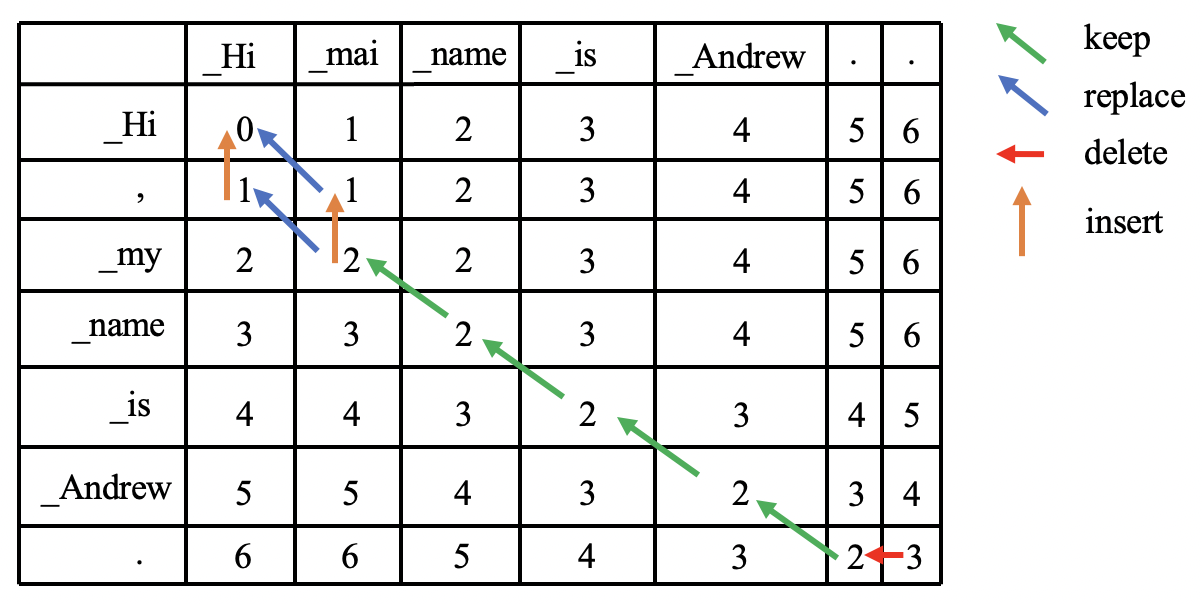
\includegraphics[width=\linewidth]{images/backtracking.png}
  \caption{Матрица Левенштейна и редакционные предписания между исходной и целевой последовательностями. Можно заметить, что существует несколько вариантов редакионных предписаний.}
  \label{fig:backtracking}
\end{figure}

Расстояние Левенштейна между исходной и целевой последовательностями эффективно вычисляется с помощью двумерной матрицы, которая заполняется с использованием алгоритма динамического программирования. Пусть $D_{i,j}$ — это расстояние редактирования между префиксами $s_k[0..i]$ и $t_k[0..j]$ длины $i$ и $j$, при этом $D_{0,j} = 0$ и $D_{i,0} = 0$. Остальные значения определяются следующим рекуррентным соотношением:

\[
D_{i,j} = 
\begin{cases} 
    D_{i-1, j-1}, & \text{если } s_k[i] = s_k[j] \\
    1 + \min \begin{cases} 
        D_{i-1, j}, \\
        D_{i, j-1}, \\
        D_{i-1, j-1} 
    \end{cases}, & \text{иначе}
\end{cases}
\]

На рисунке~\ref{fig:backtracking} показана матрица расстояний между префиксами токенизированного исходного предложения <<Hi mai name is Andrew..>> и токенизированного целевого предложения <<Hi, my name is Andrew.>>. Расстояние Левенштейна между исходной и целевой последовательностями отображается в правом нижнем углу матрицы и равно 3.

Редакционное предписание — это последовательность правил (\textit{keep}, \textit{replace}, \textit{append}, \textit{delete}) минимальной длины, описывающая действия, необходимые для получения целевой последовательности из исходной.

Чтобы найти эталонные корректирующие преобразования, необходимо определить редакционное предписание. Как показано на рисунке~\ref{fig:backtracking}, предписание можно получить с помощью обратного прохода по рассчитанной матрице расстояний. Начиная с правого нижнего угла таблицы, строим пути ко всем соседним ячейкам, соответствующим меньшим подзадачам и меньшим расстояниям редактирования. Движение вверх соответствует вставке подслова в исходную последовательность (\textit{append}), влево — удалению подслова (\textit{delete}), по диагонали — замене (\textit{replace}) или сохранению без изменений (\textit{keep}), если подслова совпадают.

\textbf{Утв. Количество редакционных предписаний соответствует количеству путей в графе подзадач с минимальной стоимостью.}

Например, для нашего случая существует два редакционных предписания:  
\{\textit{delete} \textbf{.}; \textit{append} \textbf{\_my}; \textit{replace} \textbf{\_mai} на \textbf{,}\}  
и  
\{\textit{delete} \textbf{.}; \textit{append} \textbf{,}; \textit{replace} \textbf{\_mai} на \textbf{\_my}\}.  
Таким образом, нам необходимо определить оптимальное редакционное предписание. Ввиду краткости правила \textit{keep} опущены.

Обозначим через $EP_k = \{e_{1}, e_{2}, \ldots, e_{o_k}\}$ множество редакционных предписаний для пары последовательностей $(s_k, t_k)$, где $o_k$ — количество предписаний для $k$-й пары.

Для определения оптимального редакционного предписания для $k$-й пары учитывается схожесть подслов при применении правила \textit{replace}. Пусть $R_l \in e_l, \, l \in \{1, 2, \ldots, o_k\}$ — множество всех правил \textit{replace} с мощностью $p_l$ для произвольного предписания $e_l$:
\begin{align*}
    R_l =\{replace\_{t_1}_{i}\_{t_2}_{i}\}_{i=0}^{p_l}, 
\end{align*}
где ${t_1}_i \in s_k$, ${t_2}_i \in t_k$.

Введём метрику схожести подслов:
\[
\sigma_l = \sum_{i=0}^{p_l} \text{LevenshteinDist}({t_1}_i, {t_2}_i),
\]
где $\text{LevenshteinDist}$ — функция, вычисляющая расстояние Левенштейна между ${t_1}_i$ и ${t_2}_i$ на уровне символов в подсловах.

Оптимальное предписание $e^*_l$ выбирается как:
\[
l = \arg\min \{\sigma_1, \sigma_2, \ldots, \sigma_{o_k}\}.
\]

Это и есть эталонная последовательность корректирующих преобразований для пары $(s_k, t_k)$.

\subsection{Обучающая система и экспериментальные настройки}

В этом разделе описаны методология и возникшие в процессе построения системы трудности. Для оценки качества предлагаемого подхода использована Sequence Tagging модель GECToR, показавшая высокую эффективность в задаче исправления грамматических ошибок. Для корректного сравнения с авторами модели использованы те же данные и повторен процесс обучения с теми же параметрами.

\begin{table}[h]
  \centering
  \small 
  \begin{tabular}{c*{2}{c}c}
    \hline
    \multirow{1}{*}{\textbf{\shortstack{Датасет}}} & \multicolumn{2}{c}{\textbf{Количество предложений}} & \multirow{1}{*}{\textbf{Этап}}  \\
     & Уровень подслов  & Уровень слов & \textbf{обучения} \\
    \hline
     PIE-synthetic &  9,000,000 & 9,000,000 & I \\
     Lang-8 & 787,613 & 947,344 & II  \\
     NUCLE & 51,929 & 56,958 & II  \\
     FCE & 25,968 & 34,490 & II \\
     W\&I+LOCNESS & 21,828 & 34,304 & II, III \\
    \hline
  \end{tabular}
 \caption{Наборы данных на каждом этапе обуччения с соответствующим количеством предложений: в исследовании~\cite{b15} на уровне слов и в нашем исследовании на уровне подслов.}
  \label{tab:data}
\end{table}

\subsection{Описание данных}

В таблице~\ref{tab:data} представлены статистики данных, использованных в исследовании~\cite{b15} и в нашем исследовании. Было использовано пять датасетов: PIE-synthetic~\cite{b32}, Lang-8~\cite{b33, b34}, NUCLE~\cite{b35}, FCE~\cite{b36} и W\&I+LOCNESS~\cite{b37}.

\subsubsection{Ограничения алгоритма}

Слабым местом данного подхода является то, что обратный проход использует рекурсивные вызовы для нахождения всевозможных редакционных предписаний и выбора наилучшего. Таким образом, для длинных последовательностей с большим количеством различий возникает множество путей. Для некоторых предложений не удалось найти эталонную последовательность корректирующих преобразований, и они были исключены из обучающего набора.

\subsubsection{Обучающие данные}

Как показано в таблице \ref{tab:data}, на первом этапе обучения, аналогично~\cite{b15}, использовались 9 миллионов предложений из PIE-synthetic. Однако ввиду ограничений только 6.7M предложений совпадают с теми, что использовались в~\cite{b15}. Чтобы довести общий объём до 9M, использовались оставшиеся предложения из PIE-synthetic.

Что касается реальных данных, из таблицы \ref{tab:data} видно, что использовалось только 78\% от общего объёма. Эти данные применялись для дообучения на этапах II и III.

\subsubsection{Данные для оценки}

Для сравнения качества работы моделей использовались те же тестовые наборы, что и в~\cite{b15} --- CoNLL-2014 и BEA-2019. В процессе оценки применялись метрики $M^2$ и ERRANT соответственно.

\begin{table}[h]
  \centering
  \small 
  \begin{tabular}{c*{2}{c}cc}
    \hline
    \multirow{2}{*}{\textbf{\shortstack{Этап \\ обучения}}} & \multicolumn{2}{c}{\textbf{Уровень слов}} & \multicolumn{2}{c}{\textbf{Уровень подслов}} \\
     & Количество эпох & Размер батча & Количество эпох & Размер батча \\
    \hline
     I & 20 & 256 & 20 & 32 \\
     II & 9 & 128 & 7 & 16 \\
     III & 4 & 128 & 1 & 16 \\
    \hline
  \end{tabular}
 \caption{Лучшие эпохи на каждом этапе обучения модели XLNet в~\cite{b15} на уровне слов и в нашем исследовании на уровне подслов с соответствующими размерами батча.}
  \label{tab:epochs}
\end{table}

% \begin{table*}[h]
%   \centering
%   \begin{tabular}{lcccccc}
%     \hline
%     \multirow{2}{*}{Модель} & \multicolumn{3}{c}{\textbf{CoNLL-2014 (тест)}} & \multicolumn{3}{c}{\textbf{BEA-2019 (тест)}} \\
%      & P & R & $F_{0.5}$ & P & R & $F_{0.5}$ \\
%     \hline
%     GECToR (подсловный уровень + XLNet) & 72.3 & 40.4 & 62.4 & 70.5 & 41.6 & 61.9 \\
%     \hline
%     GECToR (словесный уровень + BERT) & 72.1 & \textbf{42.0} & 63.0 & 71.5 & \textbf{55.7} & 67.6 \\ 
%     GECToR (словесный уровень + RoBERTa) & 73.9 & 41.5 & 64.0 & 77.2 & 55.1 & 71.5 \\
%     GECToR (словесный уровень + XLNet) & \textbf{77.5} & 40.1 & \textbf{65.3} & \textbf{79.2} & 53.9 & \textbf{72.4} \\
%     \hline
%   \end{tabular}
%   \caption{Сравнение моделей на подсловном и словесном уровнях. Приведены $M^2$ для CoNLL-2014 и ERRANT для BEA-2019.}
%   \label{tab:result}
% \end{table*}

\begin{table*}
  \centering
  \begin{tabular}{lcccccc}
    \hline
    \multirow{2}{*}{Model} & \multicolumn{3}{c}{\textbf{CoNLL-2014}} & \multicolumn{3}{c}{\textbf{BEA-2019}} \\
     & P & R & $F_{0.5}$ & P & R & ${F}_{0.5}$ \\
    \hline
    GECToR & 72.3 & 40.4 & 62.4 & 70.5 & 41.6 & 61.9 \\
    (уровень подслов + XLNet) & & & & & & \\
    \hline
    GECToR & 72.1 & \textbf{42.0} & 63.0 & 71.5 & \textbf{55.7} & 67.6 \\ 
    (уровень слов + BERT) & & & & & & \\
    GECToR & 73.9 & 41.5 & 64.0 & 77.2 & 55.1 & 71.5 \\
    (уровень слов + RoBERTa) & & & & & & \\
    GECToR & \textbf{77.5} & 40.1 & \textbf{65.3} & \textbf{79.2} & 53.9 & \textbf{72.4} \\
    (уровень слов + XLNet) & & & & & & \\
    % GECToR & 78.2 & 41.5 & 66.5 & 78.9 & 58.2 & 73.6 \\
    % (word-level + BERT + RoBERTa + XLNet) & & & & & & \\
    \hline
  \end{tabular}
  \caption{Сравнение работы моделей на уровне слов и на уровне подслов. Приведены оценки $M^2$ для CoNLL-2014 (тест) и ERRANT для BEA-2019 (тест).}
  \label{tab:result}
\end{table*}


\subsection{Обучение модели}

Архитектура модели GECToR состоит из кодировщика на базе архитектуры “Трансформер” и двух линейных классификаторов. Первый классификатор предсказывает наличие ошибки в каждом подслове. Второй классификатор выбирает конкретное правило из словаря для исправления подслова или оставляет его без изменений, если наиболее вероятное правило --- \textit{keep}.

Если максимальная вероятность первого классификатора по предложению ниже определённого порога, предложение не подлежит исправлению. В~\cite{b15} этот порог равен 0.66. В нашем исследовании эмпирическим путем было подобрано оптимальное значение 0.05.

\subsubsection{Исправление на уровне слов}

В~\cite{b15} словарь правил исправления был построен на уровне слов. Это означает, что несколько подслов в одном слове соотносятся с одним правилом из словаря.

В исследовании использовались два типа правил: “базовые преобразования” и “g-преобразования”. Базовые преобразования — это \textit{delete}, \textit{keep}, \textit{replace} и \textit{append}. G-преобразования --- это более сложные грамматические изменения: смена формы глагола, слияние/разде-ление слов, изменение числа существительного и др. Для построения g-трансформаций необходимо знание грамматики языка, аннотированные данные и средства сопоставления предсказанных правил с эталонными.

Весь словарь включает 5000 правил, из которых 4971 --- базовые преобразования, 29 --- g-преобразования.

\subsubsection{Исправление на уровне подслов}

В нашем подходе отсутствуют g-преобразования, что избавляет нас от необходимости вручную составлять правила. Это особенно важно для языков с богатой морфологией, для которых обобщение грамматики вручную крайне трудоёмко.

Нами был получен словарь правил на уровне подслов, используя только базовые преобразования: \textit{delete}, \textit{keep}, \textit{replace} и \textit{append}. Процесс полностью автоматический и не требует аннотированных данных, лишь параллельный корпус. Объём итогового словаря составил 25,714 правил.

\subsubsection{Параметры обучения}

В качестве кодировщика использован XLNet, так как он показал наилучшие результаты в~\cite{b15}. Процесс обучения был повторён с теми же параметрами, за исключением размера батча.

Авторы~\cite{b15} использовали размер батча 256 на первом этапе обучения и 128 на втором и третьем этапах. В нашем случае значения составили 32 и 16 соответственно. В таблице~\ref{tab:epochs} представлены лучшие эпохи для каждого этапа.



\subsection{Результаты}


Как показано в таблице~\ref{tab:result}, результаты были получены на наборах данных CoNLL-2014 (тест) и BEA-2019 (тест) с использованием соответствующих метрик --- $M^{2}$-scorer и ERRANT. 

На наборе данных CoNLL-2014 наша модель на уровне подслов показывает конкурентоспособный результат $F_{0.5} = 62.4$ по сравнению с $F_{0.5} = 65.3$ для модели на уровне слов из работы~\cite{b15}. Более того, наша модель на уровне подслов немного превосходит оригинальную модель по метрике полноты: $R = 40.4$ против $R = 40.1$.

На наборе данных BEA-2019 наша модель не смогла приблизиться к результатам оригинальной модели, однако всё ещё демонстрирует достаточно высокий показатель $F_{0.5} = 61.9$. Как видно, модель показывает относительно низкую полноту, что можно объяснить тем, что был использован не весь синтетический корпус данных. 

Тем не менее, было показано достижение сравнимых результатов, используя обучение без учителя. Важно отметить, что данный подход является независимым и может быть адаптирован к любому языку с использованием словаря на уровне подслов.


\newpage

\section{Заключение}

В данной работе рассматриваются два взаимодополняющих исследования, посвящённых задаче исправления грамматических ошибок, с фокусом на морфологически сложные языки с ограниченными ресурсами. В отличие от английского языка, для которого данная задача изучена достаточно хорошо, языки с богатой морфологией, такие как русский, остаются недостаточно исследованными из-за дефицита размеченных данных и сложности коррекции ошибок в подобных языковых контекстах.

В первом исследовании представлена интерпретируемая и эффективная система исправления ошибок в русских текстах, основанная на правилах и синтетическом наборе обучающих данных. Используя эффективную архитектуру GECToR, система продемонстрировала высокую точность на синтетических данных $F_{0.5}$ = 82,5 и показала способность к обобщению на реальных текстах $F_{0.5}$ = 22,2, превзойдя базовые модели, не обученные напрямую на таких данных. Перспективы улучшения включают расширение словаря корректирующих правил, дообучение на дополнительных датасетах и эксперименты с различными архитектурами для повышения качества исправлений.

Второе исследование предлагает полностью неконтролируемый подход к исправлению грамматических ошибок, не требующий ручной разметки данных или языково-специфичных правил. Метод основан на базовых преобразованиях на уровне подслов и использовании выравнивания по Левенштейну для генерации исправлений. Продемонстрировав эффективность для английского языка, $F_{0.5}$ = 62,4 на CoNLL-2014 и $F_{0.5}$ = 61,9 на BEA-2019, подход показал свою конкурентоспособность. Его применение особенно перспективно для малоресурсных языков, где ощущается острый дефицит размеченных данных. Дальнейшие исследования могут быть направлены на адаптацию метода к другим языкам, а также на изучение влияния различных архитектур “Трансформер” и стратегий токенизации на качество исправлений.

Вместе эти исследования демонстрируют перспективность как гибридных (основанных на правилах), так и полностью неконтролируемых подходов для решения задачи исправления грамматических ошибок в условиях ограниченных языковых ресурсов. Если первая работа подтверждает эффективность синтетических данных и структурированных корректирующих правил, то вторая доказывает возможность достижения конкурентоспособных результатов без использования размеченных данных. 


% Выводы


% Библиографические ссылки
\newpage


\begin{thebibliography}{99}

\bibitem{b1}
Rozovskaya A., Roth D. Grammatical Error Correction: Machine Translation and Classifiers // Proceedings of the 54th Annual Meeting of the Association for Computational Linguistics (Volume 1: Long Papers). — Berlin, Germany: Association for Computational Linguistics, 2016. — P. 2205–2215.

\bibitem{b2}
Yuan Z., Stahlberg F., Rei M., Byrne B., Yannakoudakis H. Neural and FST-based approaches to grammatical error correction // Proceedings of the Fourteenth Workshop on Innovative Use of NLP for Building Educational Applications. — Florence, Italy: Association for Computational Linguistics, 2019. — P. 228–239.

\bibitem{b3}
Bryant C., Ng H.T. How Far are We from Fully Automatic High Quality Grammatical Error Correction? // Proceedings of the 53rd Annual Meeting of the Association for Computational Linguistics. — Beijing, China: Association for Computational Linguistics, 2015. — P. 697–707.

\bibitem{b4}
Rajput D. Review on recent developments in frequent itemset based document clustering, its research trends and applications // International Journal of Data Analysis Techniques and Strategies. — 2019. — Vol. 11. — P. 176–195.

\bibitem{b5}
Flickinger D., Yu J. Toward More Precision in Correction of Grammatical Errors // Proceedings of the Seventeenth Conference on Computational Natural Language Learning: Shared Task. — Sofia, Bulgaria: Association for Computational Linguistics, 2013. — P. 68–73.

\bibitem{b6}
Yuan X., Pham D., Davidson S., Yu Z. ErAConD: Error Annotated Conversational Dialog Dataset for Grammatical Error Correction // Proceedings of the 2022 Conference of the North American Chapter of the Association for Computational Linguistics: Human Language Technologies. — Seattle, USA: Association for Computational Linguistics, 2022. — P. 76–84.

\bibitem{b7}
Lee J.S.Y., Seneff S. An analysis of grammatical errors in non-native speech in English // 2008 IEEE Spoken Language Technology Workshop. — 2008. — P. 89–92.

\bibitem{b8}
Zhuravlev K., Rudakov K., Inyakin A., et al. The system of recognition of intellectual text reuse “Antiplagiat” // Mathematical methods of pattern recognition: 12th All-Russian conference: Collection of reports. — Moscow: MAKS Press, 2005. — P. 329–332.

\bibitem{b9}
Keck C.M. How Do University Students Attempt to Avoid Plagiarism? A Grammatical Analysis of Undergraduate Paraphrasing Strategies // Writing \& Pedagogy. — 2010. — Vol. 2. — P. 193–222.

\bibitem{b10}
Zhang W.E., Sheng Q.Z., Alhazmi A., Li C. Adversarial Attacks on Deep-Learning Models in Natural Language Processing: A Survey // ACM Transactions on Intelligent Systems and Technology. — 2020. — Vol. 11, No. 3. — Art. 24. — P. 1–41.

\bibitem{b11}
Ng H.T., Wu S.M., Briscoe T., et al. The CoNLL-2014 Shared Task on Grammatical Error Correction // Proceedings of the Eighteenth Conference on Computational Natural Language Learning: Shared Task. — Baltimore, MD: Association for Computational Linguistics, 2014. — P. 1–14.

\bibitem{b12}
Rozovskaya A., Roth D. Grammar Error Correction in Morphologically Rich Languages: The Case of Russian // Transactions of the Association for Computational Linguistics. — 2019. — Vol. 7. — P. 1–17.

\bibitem{b13}
Rothe S., Mallinson J., Malmi E., Krause S., Severyn A. A Simple Recipe for Multilingual Grammatical Error Correction // Proceedings of the 59th Annual Meeting of the Association for Computational Linguistics and the 11th International Joint Conference on Natural Language Processing (Volume 2: Short Papers). — Online: Association for Computational Linguistics, 2021. — P. 702–707.

\bibitem{b14}
Grundkiewicz R., Junczys-Dowmunt M., Heafield K. Neural Grammatical Error Correction Systems with Unsupervised Pre-training on Synthetic Data // Proceedings of the Fourteenth Workshop on Innovative Use of NLP for Building Educational Applications. — Florence, Italy: Association for Computational Linguistics, 2019. — P. 252–263.

\bibitem{b15}
Omelianchuk K., Atrasevych V., Chernodub A., Skurzhanskyi O. GECToR – Grammatical Error Correction: Tag, Not Rewrite // Proceedings of the Fifteenth Workshop on Innovative Use of NLP for Building Educational Applications. — Seattle, WA, USA → Online: Association for Computational Linguistics, 2020. — P. 163–170.

\bibitem{b16}
Malmi E., Krause S., Rothe S., Mirylenka D., Severyn A. Encode, Tag, Realize: High-Precision Text Editing // Proceedings of the 2019 Conference on Empirical Methods in Natural Language Processing and the 9th International Joint Conference on Natural Language Processing (EMNLP-IJCNLP). — Hong Kong: Association for Computational Linguistics, 2019. — P. 5054–5065.

\bibitem{b17}
Vaswani A., Shazeer N., Parmar N., et al. Attention is All You Need // Advances in Neural Information Processing Systems. — 2017. — Vol. 30.


\bibitem{b18}
Devlin J., Chang M.-W., Lee K., Toutanova K.  
BERT: Pre-training of Deep Bidirectional Transformers for Language Understanding // Proceedings of the 2019 Conference of the North American Chapter of the Association for Computational Linguistics: Human Language Technologies, Volume 1 (Long and Short Papers). — Minneapolis, Minnesota: Association for Computational Linguistics, 2019. — P. 4171–4186. — DOI: \url{10.18653/v1/N19-1423}.

\bibitem{b19}
Liu Y., Ott M., Goyal N., Du J., Joshi M., Chen D., Levy O., Lewis M., Zettlemoyer L., Stoyanov V.  
RoBERTa: A Robustly Optimized BERT Pretraining Approach [Электронный ресурс]. — 2019. — Режим доступа: \url{http://arxiv.org/abs/1907.11692} (дата обращения: 03.06.2025)


\bibitem{b20}
Yang Z., Dai Z., Yang Y., Carbonell J., Salakhutdinov R., Le Q. V.  
XLNet: generalized autoregressive pretraining for language understanding // Proceedings of the 33rd International Conference on Neural Information Processing Systems. — Red Hook, NY, USA: Curran Associates Inc., 2019. — Article No. 517. — 11 p.

\bibitem{b21}
Khabutdinov I. A., Chashchin A. V., Grabovoy A. V., Kildyakov A. S., Chekhovich U. V.  
RuGECToR: Rule-Based Neural Network Model for Russian Language Grammatical Error Correction // Program. Comput. Softw. — 2024. — Vol. 50, no. 4. — P. 315–321. — DOI: \href{https://doi.org/10.1134/S0361768824700129}{10.1134/S0361768824700129}.

\bibitem{b22}
Kudo T., Richardson J.  
SentencePiece: A simple and language independent subword tokenizer and detokenizer for Neural Text Processing // In: Proceedings of the 2018 Conference on Empirical Methods in Natural Language Processing: System Demonstrations. — Brussels, Belgium: Association for Computational Linguistics, 2018. — P. 66–71. — DOI: \href{https://doi.org/10.18653/v1/D18-2012}{10.18653/v1/D18-2012}.

\bibitem{b23}
Korobov M. Morphological Analyzer and Generator for Russian and Ukrainian Languages // Analysis of Images, Social Networks and Texts. — Springer, 2015. — Vol. 542. — P. 320–332.

\bibitem{b24}
Open source collection of school essays [Электронный ресурс]. — Режим доступа: \url{https://www.kritika24.ru} (дата обращения: 07.11.2022).

\bibitem{b25}
Open source collection of literary works [Электронный ресурс]. — Режим доступа: \url{https://proza.ru} (дата обращения: 07.11.2022).

\bibitem{b26}
Trinh V.A., Rozovskaya A. New Dataset and Strong Baselines for the Grammatical Error Correction of Russian // Findings of the Association for Computational Linguistics: ACL-IJCNLP 2021. — Online: Association for Computational Linguistics, 2021. — P. 4103–4111.

\bibitem{b27}
Lyashevskaya O., Sharov S. Frequency Dictionary of the Modern Russian Language (based on the materials of the National Corpus of the Russian Language) [in Russian]. — Moscow: Azbukovnik, 2009. — 21 p.

\bibitem{b28}
Kingma D., Ba J.  
Adam: A Method for Stochastic Optimization // International Conference on Learning Representations (ICLR). — 2015. — arXiv:1412.6980.

\bibitem{b29}
Limisiewicz T., Balhar J., Mareček D.  
Tokenization Impacts Multilingual Language Modeling: Assessing Vocabulary Allocation and Overlap Across Languages // *Findings of the Association for Computational Linguistics: ACL 2023*. — Toronto, Canada: Association for Computational Linguistics, 2023. — P. 5661–5681. — DOI: 10.18653/v1/2023.findings-acl.350.

\bibitem{b30}
Asvarov A., Grabovoy A.  
The Impact of Multilinguality and Tokenization on Statistical Machine Translation // *Proceedings of the 2024 Conference*. — 2024. — P. 149–157. — DOI: 10.23919/FRUCT61870.2024.10516416.

\bibitem{b31}
Dahlmeier D., Ng H.T.  
Better Evaluation for Grammatical Error Correction // *Proceedings of the 2012 Conference of the North American Chapter of the Association for Computational Linguistics: Human Language Technologies*. — Montréal, Canada: Association for Computational Linguistics, 2012. — P. 568–572.

\bibitem{b32}
Awasthi A., Sarawagi S., Goyal R., Ghosh S., Piratla V.  
Parallel Iterative Edit Models for Local Sequence Transduction // *Proceedings of the 2019 Conference on Empirical Methods in Natural Language Processing and the 9th International Joint Conference on Natural Language Processing (EMNLP-IJCNLP)*. — Hong Kong, China: Association for Computational Linguistics, 2019. — P. 4259–4269. — DOI: 10.18653/v1/D19-1435.

\bibitem{b33}
Mizumoto T., Komachi M., Nagata M., Matsumoto Y.  
Mining revision log of language learning SNS for automated Japanese error correction of second language learners // *Proceedings of the 5th International Joint Conference on Natural Language Processing*. — 2011. — P. 147–155.


\bibitem{b34}
Rothe S., Mallinson J., Malmi E., Krause S., Severyn A.  
A Simple Recipe for Multilingual Grammatical Error Correction // *Proceedings of the 59th Annual Meeting of the Association for Computational Linguistics and the 11th International Joint Conference on Natural Language Processing (Volume 2: Short Papers)*. — 2021. — P. 702–707. — DOI: 10.18653/v1/2021.acl-short.89.

\bibitem{b35}
Dahlmeier D., Ng H. T., Wu S.  
Building a Large Annotated Corpus of Learner English: The NUS Corpus of Learner English~//  
\textit{Proceedings of the Eighth Workshop on Innovative Use of NLP for Building Educational Applications}. — Atlanta, Georgia: Association for Computational Linguistics, 2013. — P.~22--31. — URL: \href{https://aclanthology.org/W13-1703}{aclanthology.org/W13-1703}.

\bibitem{b36}
Yannakoudakis H., Briscoe T., Medlock B.  
A New Dataset and Method for Automatically Grading ESOL Texts~//  
\textit{Proceedings of the 49th Annual Meeting of the Association for Computational Linguistics: Human Language Technologies}. — Portland, Oregon, USA: Association for Computational Linguistics, 2011. — P.~180--189. — URL: \href{https://aclanthology.org/P11-1019}{aclanthology.org/P11-1019}.

\bibitem{b37}
Bryant C., Felice M., Andersen {\O}.E., Briscoe T.  
The BEA-2019 Shared Task on Grammatical Error Correction~//  
\textit{Proceedings of the Fourteenth Workshop on Innovative Use of NLP for Building Educational Applications}. — Florence, Italy: Association for Computational Linguistics, 2019. — P.~52--75.  
DOI: \href{https://doi.org/10.18653/v1/W19-4406}{10.18653/v1/W19-4406}.  
URL: \href{https://aclanthology.org/W19-4406}{aclanthology.org/W19-4406}.



\end{thebibliography}





% Приложения
%\newpage

\appendix
\setcounter{theorem}{0}
\section{Теорема (Грабовой 2019)}\label{ProofTheorem1}
\begin{theorem}\label{th:1} 
Пусть задано множество подпространств~$\mathbb{W}$ пространства~$\mathbb{R}^{n}$, каждое подпространство которого задается базисом~$\mathbf{W}_i\in \mathbf{W}$, тогда функция расстояния~$\rho\left(\textbf{W}_1, \textbf{W}_2\right)$ является метрикой заданой на множестве базисов~$\mathbf{W}$:
\begin{equation}
\label{eq:th2:1}
\begin{aligned}
\rho\left(\textbf{W}_1, \textbf{W}_2\right) = \max\left(\max_{\textbf{e}_2 \in \textbf{W}_2} h_{1}\left(\textbf{e}_2\right), \max_{\textbf{e}_1 \in \textbf{W}_1} h_{2}\left(\textbf{e}_1\right)\right),
\end{aligned}
\end{equation}
где~$\textbf{e}_i$ это базисный вектор из~$\textbf{W}_i$,~$h_i\left(\textbf{e}\right)$ является расстоянием от вектора~$\textbf{e}$ до пространства заданого базисом~$\textbf{W}_i$.
\end{theorem}
\begin{proof}
Для доказательства данной теоремы, нужно показать, что функция~$\rho$ удовлетворяет трем свойствам метрики.

Функция~$\rho$ удовлетворяет первому свойству метрики:
\begin{equation}
\label{eq:th2:2}
\begin{aligned}
\rho\left(\textbf{W}_1, \textbf{W}_2\right) = 0 \Leftrightarrow \textbf{W}_1 = \textbf{W}_2
\end{aligned}
\end{equation}

Функция~$\rho$ удовлетворяет второму свойству метрики:
\begin{equation}
\label{eq:th2:3}
\begin{aligned}
\rho\left(\textbf{W}_1, \textbf{W}_2\right) = \rho\left(\textbf{W}_2, \textbf{W}_1\right)
\end{aligned}
\end{equation}

Докажем, что функция~$\rho$ удовлетворяет удовлетворяет неравенству треугольника:
\begin{equation}
\label{eq:th2:4}
\begin{aligned}
\rho\left(\textbf{W}_1, \textbf{W}_2\right) \leq \rho\left(\textbf{W}_1, \textbf{W}_3\right) + \rho\left(\textbf{W}_3, \textbf{W}_2\right)
\end{aligned}
\end{equation}

Для доказательства неравенства треугольника докажем неравенства:
\begin{equation}
\label{eq:th2:5}
\begin{aligned}
\max_{\textbf{e}_1 \in \textbf{W}_1}h_{2}\left(\textbf{e}_1\right) \leq 
\max_{\textbf{e}_1\in \textbf{W}_1}h_{3}\left(\textbf{e}_1\right)+
\max_{\textbf{e}_3 \in \textbf{W}_3}h_{2}\left(\textbf{e}_3\right) \\
\max_{\textbf{e}_2 \in \textbf{W}_2}h_{1}\left(\textbf{e}_2\right) \leq 
\max_{\textbf{e}_2\in \textbf{W}_2}h_{3}\left(\textbf{e}_2\right)+
\max_{\textbf{e}_3 \in \textbf{W}_3}h_{1}\left(\textbf{e}_3\right)
\end{aligned}
\end{equation}

Используя Лемму~\ref{lem:1} доказательство неравенства (\ref{eq:th2:5}) сводится к доказательства неравенства:
\begin{equation}
\label{eq:th2:6}
\begin{aligned}
\max_{\substack{\textbf{a} \in \textbf{W}_1 \\ \left|\textbf{a}\right| \leq 1}}h_{2}\left(\textbf{a}\right) \leq 
\max_{\substack{\textbf{a} \in \textbf{W}_1 \\ \left|\textbf{a}\right| \leq 1}}h_{3}\left(\textbf{a}\right)+
\max_{\substack{\textbf{c} \in \textbf{W}_3 \\ \left|\textbf{c}\right| \leq 1}}h_{2}\left(\textbf{c}\right),
\end{aligned}
\end{equation}
где~$\textbf{a}, \textbf{c}$ произвольные элементы из соответствующих подпространств. 

Подставив в выражение~(\ref{eq:th2:6}) выражение для~$h_i\left(\textbf{a}\right)$, получаем следующее неравенство:
\begin{equation}
\label{eq:th2:7}
\begin{aligned}
\max_{\substack{\textbf{a} \in \textbf{W}_1 \\ \left|\textbf{a}\right| \leq 1}} \min_{\substack{\textbf{b} \in \textbf{W}_2 \\ \left|\textbf{b}\right| \leq 1}}||\textbf{a} - \textbf{b}|| \leq 
\max_{\substack{\textbf{a} \in \textbf{W}_1 \\ \left|\textbf{a}\right| \leq 1}} \min_{\substack{\textbf{c} \in \textbf{W}_3 \\ \left|\textbf{b}\right| \leq 1}}||\textbf{a} - \textbf{c}||+
\max_{\substack{\textbf{c} \in \textbf{W}_3 \\ \left|\textbf{c}\right| \leq 1}} \min_{\substack{\textbf{b} \in \textbf{W}_2 \\ \left|\textbf{b}\right| \leq 1}}||\textbf{c} - \textbf{b}||.
\end{aligned}
\end{equation}

Неравенство~(\ref{eq:th2:7}) следует из Леммы~\ref{lem:2}. Из выполнения неравенства~(\ref{eq:th2:7}) следует выполнение неравенств~(\ref{eq:th2:5}).
Докажем неравенство треугольника~(\ref{eq:th2:4}) используя неравенства~(\ref{eq:th2:5}). Для удобства введем следующие обозначения:
\begin{equation}
\label{eq:th2:8}
\begin{aligned}
\max_{\textbf{e}_i \in \textbf{W}_i} h_{\textbf{W}_j}\left(\textbf{e}_i\right) = h_{i}^{j}.
\end{aligned}
\end{equation}

Из истинности неравенства~(\ref{eq:th2:7}) в обозначениях~(\ref{eq:th2:8}) следует истинность следующих неравенств:
 
\begin{equation}
\label{eq:th2:9}
\begin{aligned}
\quad h_{1}^{2} \leq h_{1}^{3} + h_{3}^{2} \leq \max\left(h_{1}^{3}, h_{3}^{1}\right) + \max\left(h_{3}^{2}, h_{2}^{3}\right)\\
\quad h_{2}^{1} \leq h_{2}^{3} + h_{3}^{1} \leq \max\left(h_{2}^{3}, h_{3}^{2}\right) + \max\left(h_{3}^{1}, h_{1}^{3}\right)\\
\end{aligned}
\end{equation}

Из уравнения~(\ref{eq:th2:9}) следует выполнение неравенства:
\begin{equation}
\label{eq:th2:10}
\begin{aligned}
\max\left(h_{1}^{2}, h_{2}^{1}\right) \leq  \max\left(h_{1}^{3}, h_{3}^{1}\right) + \max\left(h_{3}^{2}, h_{2}^{3}\right)\\
\end{aligned}
\end{equation}

Доказательство неравенства~(\ref{eq:th2:10}) указывает на выполнение неравенства треугольника для функции~$\rho$, что завершает доказательство того, что~$\rho$ является метрикой.

\end{proof}


\begin{lemma} \label{lem:1} 
Пусть заданы два подпространства~$\mathbb{X}, \mathbb{Y} \subset \mathbb{R}^{n}$, которые задаются базисами~$\textbf{W}_1$ и~$\textbf{W}_2$, тогда справедливо следующее условие:

\begin{equation}
\label{eq:l1:1}
\begin{aligned}
\max_{\textbf{a} \in \mathbb{X}:~\left|\textbf{a}\right|\leq 1}h_2\left(\textbf{a}\right)
\end{aligned}
\end{equation}
где~$h_i\left(\textbf{a}\right)$ является расстоянием от вектора~$\textbf{a}$ до пространства заданого базисом~$\textbf{W}_i$.
\end{lemma}

\begin{proof}
\begin{equation}
\label{eq:l1:2}
\begin{aligned}
\max_{\textbf{a} \in \mathbb{X}:~\left|\textbf{a}\right|\leq 1}h_2\left(\textbf{a}\right) = \max_{\textbf{a} \in \mathbb{X}:~\left|\textbf{a}\right|\leq 1}\left|\textbf{a}-\sum_{i}\langle \textbf{e}^i_2, \textbf{a} \rangle\textbf{e}^i_2 \right| = \\ 
=\max_{\{\alpha_j\}_{j}:~\sum\alpha_j^2\leq 1}\left|\sum_{j}\alpha_j\textbf{e}^{j}_1-\sum_{i}\langle \textbf{e}^i_2, \sum_{j}\alpha_j\textbf{e}^{j}_1 \rangle\textbf{e}^i_2 \right| =\\
= \max_{\{\alpha_j\}_{j}:~\sum\alpha_j^2\leq 1}\left|\sum_{j}\alpha_j\left(\textbf{e}_3^j - \sum_{i}\langle\textbf{e}_3^j,\textbf{e}_2^i\rangle\textbf{e}_2^i\right)\right|,
\end{aligned}
\end{equation}
где в выражении~(\ref{eq:l1:2}) максимум очевидно достигается на~$j$-ом базисном векторе для которого выражение в скобках является максимальным.
\end{proof}




\begin{lemma} \label{lem:2} 
Пусть заданы подпространства~$\mathbb{X}, \mathbb{Y}, \mathbb{Z} \subset \mathbb{R}^{n}$, которые задаются базисами~$\textbf{W}_1, \textbf{W}_2, \textbf{W}_3$ соответственно, тогда справедливо следующее условие:

\begin{equation}
\label{eq:l2:1}
\begin{aligned}
\max_{\substack{\textbf{x} \in \mathbb{X} \\ \left|\textbf{x}\right|\leq 1}}\min_{\substack{\textbf{y} \in \mathbb{Y} \\ \left|\textbf{y}\right|\leq 1}}||\textbf{x}-\textbf{y}||\leq 
\max_{\substack{\textbf{x} \in \mathbb{X} \\ \left|\textbf{x}\right|\leq 1}}\min_{\substack{\textbf{z} \in \mathbb{Z} \\ \left|\textbf{z}\right|\leq 1}}||\textbf{x}-\textbf{z}|| + 
\max_{\substack{\textbf{z} \in \mathbb{Z} \\ \left|\textbf{z}\right|\leq 1}}\min_{\substack{\textbf{y} \in \mathbb{Y} \\ \left|\textbf{y}\right|\leq 1}}||\textbf{z}-\textbf{y}||.
\end{aligned}
\end{equation}
\end{lemma}

\begin{proof} 
\begin{equation}
\label{eq:l2:2}
\begin{aligned}
\max_{\substack{\textbf{x} \in \mathbb{X} \\ \left|\textbf{x}\right|\leq 1}}\min_{\substack{\textbf{y} \in \mathbb{Y} \\ \left|\textbf{y}\right|\leq 1}}||\textbf{x}-\textbf{y}||\leq
\max_{\substack{\textbf{x} \in \mathbb{X} \\ \left|\textbf{x}\right|\leq 1}}\min_{\substack{\textbf{y} \in \mathbb{Y} \\ \left|\textbf{y}\right|\leq 1}}\left(||\textbf{x}-\textbf{z}|| + ||\textbf{z} - \textbf{y}||\right) = \\
\max_{\substack{\textbf{x} \in \mathbb{X} \\ \left|\textbf{x}\right|\leq 1}}||\textbf{x}-\textbf{z}|| + \min_{\substack{\textbf{y} \in \mathbb{Y} \\ \left|\textbf{y}\right|\leq 1}}||\textbf{z} - \textbf{y}|| = \max_{\substack{\textbf{x} \in \mathbb{X} \\ \left|\textbf{x}\right|\leq 1}}\min_{\substack{\textbf{z} \in \mathbb{Z} \\ \left|\textbf{z}\right|\leq 1}}||\textbf{x}-\textbf{z}|| + \min_{\substack{\textbf{y} \in \mathbb{Y} \\ \left|\textbf{y}\right|\leq 1}}||\textbf{z} - \textbf{y}|| \leq \\
\leq \max_{\substack{\textbf{x} \in \mathbb{X} \\ \left|\textbf{x}\right|\leq 1}}\min_{\substack{\textbf{z} \in \mathbb{Z} \\ \left|\textbf{z}\right|\leq 1}}||\textbf{x}-\textbf{z}|| + 
\max_{\substack{\textbf{z} \in \mathbb{Z} \\ \left|\textbf{z}\right|\leq 1}}\min_{\substack{\textbf{y} \in \mathbb{Y} \\ \left|\textbf{y}\right|\leq 1}}||\textbf{z}-\textbf{y}||.
\end{aligned}
\end{equation}
\end{proof}

\end{document}
